\section{Column generation cycle cover algorithm}

We saw in Chapter \ref{chapter:te} that column generation seemed to be a good framework to solve segment routing
problems. In this section we propose a column generation algorithm for computing lower bounds on the number of sr-cycles in a
minimum sr-cycle cover of a network. We also show how to derive from it an heuristic algorithm for Problem \ref{prob:min-cycle-cover}.

It is straightforward to express a MIP formulation for Problem \ref{prob:min-cycle-cover}. We define binary
variables $x_{\sr{c}}$ such that $x_{\sr{c}} = 1$ if and only if $\sr{c}$ is used in the cover. These variables
will be defined for every $\sr{c} \in \mathcal{C}^k_s$ where $k$ and $s$ are given as input. 

In terms of objective function, since we want to minimize the number of cycles in the cover, we can achieve this
by minimizing $\sum_{\sr{c} \in \mathcal{C}^k_s} x_{\sr{c}}$. This is so because this sum counts how many cycles
are used in the solution. For the constraints it is quite simple as well. We simply need to ensure that for each
edge $e \in E(G)$, there is at least one sr-cycle covering it, that is, there is at least one $\sr{c}$ such that
$x_{\sr{c}} = 1$ and $e \in E(\sr{c})$. We define the following identify function to simplify the expression of this constraints.

\begin{definition}
Given a network $G$ we define a function $I : \mathcal{P} \times E(G) \rightarrow \{0, 1\}$ such that
$I(\sr{p}, e) = 1$ if and only if $e \in E(\sr{p})$.
\end{definition}

\begin{center}
\begin{tabular}{crcllr}
\multicolumn{5}{l}{$\ccPrimalMip(G, k, s)$} \\[0.5cm] 
$\mathbf{min}$ & $\displaystyle \sum_{\sr{c} \in \mathcal{C}^k_s} x_{\sr{c}}$ & & & & \\[0.5cm]
$\textbf{s.t.}$ & $\displaystyle \sum_{\sr{c} \in \mathcal{C}^k_s} I(\sr{c}, e) \cdot x_{\sr{c}}$  & $\geq$ & $1$ & $\forall e \in E(G)$ & \\[0.5cm]
                & $x_{\sr{c}}$ & $\in$ & $\{0, 1\}$ & $\forall \sr{c} \in \mathcal{C}^k_s$
\end{tabular}
\end{center}

\subsection{Column generation}

We follow the same process that we did in Chapter \ref{chapter:te} to develop the column generation algorithm
for the minimum sr-cycle cover problem. Recall that CG is a technique for solving a LP and we have a MIP.
The first step is then to consider the LP-relaxation of $\ccPrimalMip$ and compute its dual.

\begin{center}
\begin{tabular}{crcllr}
\multicolumn{5}{l}{$\ccPrimalLp(G, k, s)$} \\[0.5cm] 
$\mathbf{min}$ & $\displaystyle \sum_{\sr{c} \in \mathcal{C}^k_s} x_{\sr{c}}$ & & & & \\[0.5cm]
$\textbf{s.t.}$ & $\displaystyle \sum_{\sr{c} \in \mathcal{C}^k_s} I(\sr{c}, e) \cdot x_{\sr{c}}$   & $\geq$ & $1$ & $\forall e \in E(G)$ & (P1) \\[0.5cm]
                & $x_{\sr{c}}$ & $\geq$  & $0$ & $\forall \sr{c} \in \mathcal{C}^k_s$
\end{tabular}
\end{center}

As before, the most natural relaxation would be to set $x_{\sr{c}} \in [0, 1]$ but our objective function guarantees that
this is equivalent to $x_{\sr{c}} \geq 0$. We chose the second one because it is equivalent and easier to work with.
The dual is obtained by following the same systematic procedure as before. By doing so we get the following LP.

\begin{center}
\begin{tabular}{crcllr}
\multicolumn{5}{l}{$\ccDualLp(G, k, s)$} \\[0.5cm] 
$\mathbf{max}$ & $\displaystyle \sum_{e \in E(G)} y_{e}$ & & & & \\[0.5cm]
$\textbf{s.t.}$ & $\displaystyle \sum_{e \in E(G)} I(\sr{c}, e) \cdot y_e$   & $\leq$ & $1$ & $\forall \sr{c} \in \mathcal{C}^k_s$ & (D1) \\[0.5cm]
                & $y_e$ & $\geq$ & $0$ & $\forall e \in E(G)$
\end{tabular}
\end{center}

The idea to solve $\ccPrimalLp$ is again to start with a small but feasible subset of sr-cycles $C \subseteq \mathcal{C}^k_s$ and 
slowly grow it until we can prove optimality. We denote the problems restricted to $C$ by adding $C$ as an argument, that is, by
$\ccPrimalLp(G, k, s, C)$ and $\ccDualLp(G, k, s, C)$. To find a new element $\sr{c}$ to add to $C$ we need to, given an optimal
solution $y^*$ of $\ccDualLp(G, k, s, C)$, find a sr-cycle $\sr{c}$ such that

$$
\sum_{e \in E(G)} I(\sr{c}, e) \cdot y^*_e = \sum_{e \in E(\sr{c})} y^*_e > 1.
$$

Solving this directly is \NPhard~since it can be shown to be equivalent to the longest path problem. 
Instead of trying to solve this pricing problem directly, we are going to see that by slightly changing the LP formulation we can
obtain a polynomial time solvable pricing problem.

\begin{definition}
Given a network $G$ we define a function $K : \mathcal{P} \times E(G) \rightarrow \mathbb{N}$ such that
$K(\sr{p}, e)$ equals the number of times $e$ is traversed by $\sr{p}$. Formally, if $\sr{p} = \langle x_1, \ldots, x_l \rangle$
$$
K(\sr{p}, e) = \sum_{i = 2}^l I(\sp(x^2_i, x^1_{i - 1}), e) + \sum_{i = 1 : x_i = e}^l 1.
$$
\end{definition}

By replacing $I$ by $K$ in the above formulations we still get a model for Problem \ref{prob:min-cycle-cover} since, the new constraints
corresponding to $(P1)$ with $I$ replaced by $K$, will still be true if and only if every edge is covered by at least one cycle. With this change the formulations become:

\begin{center}
\begin{tabular}{crcllr}
\multicolumn{5}{l}{$\ccPrimalLpK(G, k, s)$} \\[0.5cm] 
$\mathbf{min}$ & $\displaystyle \sum_{\sr{c} \in \mathcal{C}^k_s} x_{\sr{c}}$ & & & & \\[0.5cm]
$\textbf{s.t.}$ & $\displaystyle \sum_{\sr{c} \in \mathcal{C}^k_s} K(\sr{c}, e) \cdot x_{\sr{c}}$   & $\geq$ & $1$ & $\forall e \in E(G)$ &  \\[0.5cm]
                & $x_{\sr{c}}$ & $\geq$  & $0$ & $\forall \sr{c} \in \mathcal{C}^k_s$
\end{tabular}
\end{center}

\begin{center}
\begin{tabular}{crcllr}
\multicolumn{5}{l}{$\ccDualLpK(G, k, s)$} \\[0.5cm] 
$\mathbf{max}$ & $\displaystyle \sum_{e \in E(G)} y_{e}$ & & & & \\[0.5cm]
$\textbf{s.t.}$ & $\displaystyle \sum_{e \in E(G)} K(\sr{c}, e) \cdot y_e$   & $\leq$ & $1$ & $\forall \sr{c} \in \mathcal{C}^k_s$ &  \\[0.5cm]
                & $y_e$ & $\geq$ & $0$ & $\forall e \in E(G)$
\end{tabular}
\end{center}

The pricing problem now becomes the following one.

\begin{problem}{SRCC pricing}
\label{prob:cc-pricing}
\textbf{Input:} A network $G$, $k \in \mathbb{N}$, a source node $s \in V(G)$ and values $y_e \geq 0$ for each $e \in E(G)$.

\textbf{Output:} A sr-cycle $\sr{c} \in \mathcal{C}^k_s$ such that
$$
\sum_{e \in E(G)} K(\sr{c}, e) \cdot y_e > 1
$$
or report that no such sr-cycle exists.
\end{problem}

In order to solve Problem \ref{prob:cc-pricing}, we define a sr-metric $w$ such that 
$$
w(u, v) = \sum_{e \in \sp(u, v)} y_e
$$
and
$$
w(e) = y_e.
$$

With this metric, it is easy to see can see that
$$
w(\sr{c}) = \sum_{e \in E(G)} K(\sr{c}, e) \cdot y_e.
$$

Therefore we can solve the pricing problem by computing a sr-cycle $\sr{c}$ from $s$ to $s$ of segment
cost at most $k$ such that $w(\sr{c})$ is maximum. We have already shown in Chapter \ref{chapter:sr-optimal} that 
this problem can be solved in polynomial time. Therefore, we have the following theorem.

\begin{theorem}
Problem \ref{prob:cc-pricing} can be solved in polynomial time.
\end{theorem}

To start the column generation algorithm we need a feasible solution. In order to obtain one, we run Algorithm \ref{algo:min-seg-cover2} which also gives us
suitable source node $s$ and lower bound on the segment cost $k$. If the target segment cost is lower than $k$ then we immediately know
that a feasible solution does not exist. If it does, we use the cycles produced by the minimum segment cost cycle cover algorithm as an 
initial feasible solution for the column generation algorithm.

We evaluated the runtime of the column generation algorithm over all topologies. Figure \ref{fig:cc_runtime} shows a CDF of these runtimes.
The slowest topology took about $3$ hours so solve. Most topologies are solved in a very short amount of time and $98\%$ of the topologies
are solved in under $25$ minutes. These values are very reasonable given that the probing cycle only needs to be computed when the topology changes.

\begin{figure}
\begin{center}
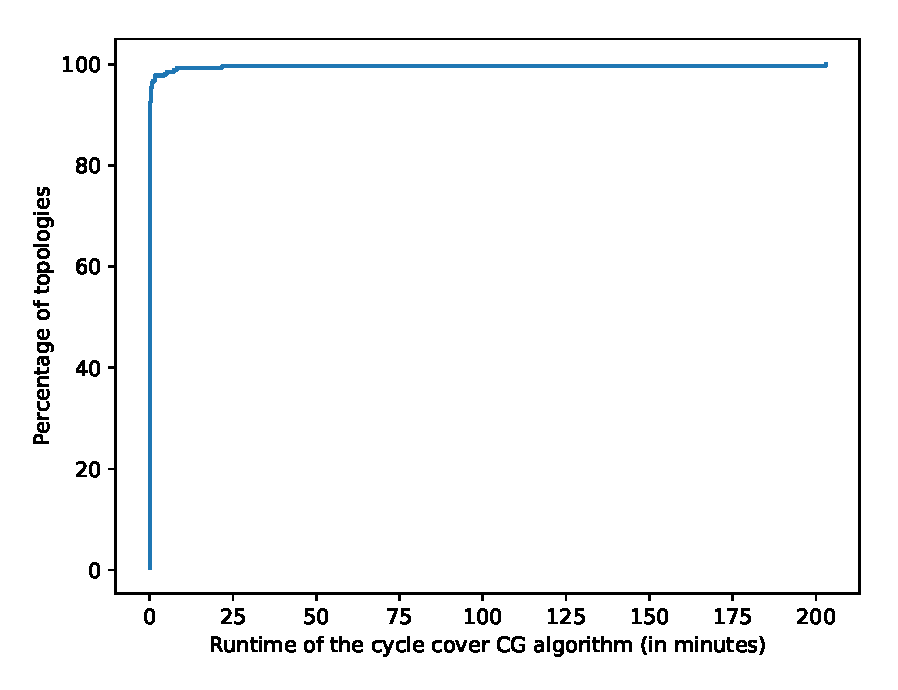
\includegraphics[width=.9\columnwidth]{./Network-lib/data/plot/minCycleCover_runtime_cdf.eps}
\end{center}
\caption{CDF of the runtime of the column generation cycle cover algorithm.}
\label{fig:cc_runtime}
\end{figure}

In the next section we will evaluate the lower bound provided by the column generation algorithm.


\subsection{Greedy algorithm}

We designed above a column generation algorithm for solving the LP relaxation of Problem \ref{prob:min-cycle-cover}. In this relaxation, an edge
can be covered fractionally by two sr-cycles or more. In this section we propose a greedy algorithm for converting these fractional solutions to proper 
solutions of Problem \ref{prob:min-cycle-cover}.

Let $C$ be the final set of sr-cycles. Our algorithm simply consists of selecting elements of $C$ 
while keeping track of the edges that are already covered until all of them are. At each step,
the sr-cycle that we selected is the sr-cycle that covers the maximum remaining uncovered edges. 

\begin{algorithm}[t]
\small
\caption{$\textsf{greedy-cc}\left( G, C \right)$}
\begin{algorithmic}[1]
%\algrule
\STATE $covered \gets \emptyset$
\STATE $cover \gets \emptyset$
\WHILE{$|U| < |E(G)|$}
  \STATE $\sr{c} \gets \sr{c} \in C \textbf{ such that } |E(\sr{c}) \cup covered| \textbf{ is maximum}$
  \STATE $cover \gets cover \cup \{ \sr{c} \}$
  \STATE $covered \gets covered \cup E(\sr{c})$
\ENDWHILE
\RETURN $cover$
\end{algorithmic}
\label{algo:greedy-cc}
\end{algorithm}

It is a well know result that this yields a logarithmic factor approximation. We prove this in the next theorem
for completeness.

\begin{theorem}
The set of cycles, $cover$, produced by Algorithm \ref{algo:greedy-cc} is such that
$$
opt_C \leq |cover| \leq \log|E(G)| \cdot opt_C
$$
where $opt_C$ is the size of a minimum over using only cycles from $C$.
\end{theorem}

\begin{proof}
Clearly, $opt_C \leq |cover|$. Let $m = |E(G)|$. 
Since the optimal solution relative to $C$ uses $opt_C$ sr-cycles, there must be at least one of them that covers at
least a fraction $1 \slash opt_C$ of the edges. If they were all below this ratio, they could not cover all edges.
Since we select the sr-cycle that covers the most uncovered edges, the first sr-cycle will cover
at least $1 \slash opt_C$ edges. Hence, after the first iteration, there are at most $m (1 - 1 \slash opt_C)$ edges left to cover. In the same way,
there must be a set that covers at least $1 \slash opt_C$ of these $m (1 - 1 \slash opt_C)$ edges. Since we select the 
sr-cycle covering the most edges, after the second iteration there are at most $m(1 - \slash opt_C)^2$ edges left. By repeating this argument,
we see that after $k$ iterations there are at most $m (1 - 1 \slash opt_C)^k$ edges left. Therefore, after $k = opt_C \log m$ iterations,
there are
$$
m (1 - 1 \slash opt_C)^{opt_C \log m} = m (1 \slash e)^{\log m} = m \cdot \frac{1}{e^{\log m}} = \frac{m}{m} = 1
$$
edges left. Hence $|cover| \leq \log m \cdot opt_C$.
\end{proof}

Ideally we would want to be able to prove that
$$
opt \leq |cover| \leq \log|E(G)| \cdot opt
$$
where $opt$ is the optimal solution over \emph{all} sr-cycles $\mathcal{C}^k_s$ but unfortunately this is not true in general.
However, since the fractional solution obtained with the column generation is a lower bound on $opt$ we can still evaluate how far
this gets us from the $opt$ in practice. Figure \ref{fig:sizes_3} shows the sizes of the minimum segment cost covers, the LP lower bound
and the sizes of the greedy covers.

\begin{figure}
\begin{center}
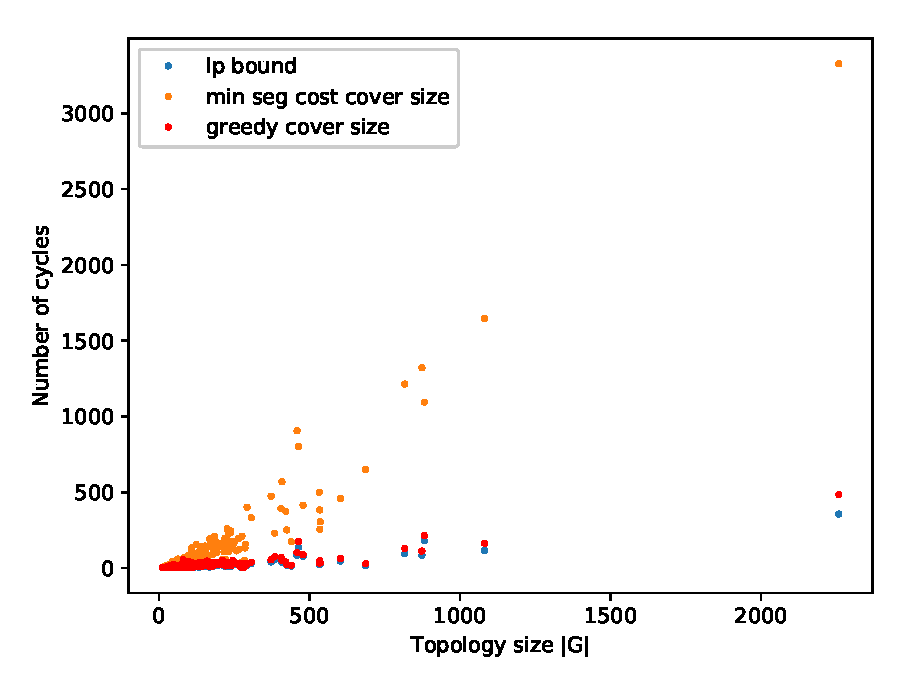
\includegraphics[width=.9\columnwidth]{./Network-lib/data/plot/minCycleCover_lowerbound.eps}
\end{center}
\caption{Lower bound, min seg cover size and greedy cover size shown by topologies size.}
\label{fig:sizes_3}
\end{figure}

We can see that the greedy solution is actually quite close to the lower bound and therefore it must also be
close to $opt$. To provide a better view of how close they are we computed a CDF of relative distance 
$$
\frac{greedy - lb}{lb}
$$
which is shown in Figure \ref{fig:cc_gap_cdf}. As a reference, with this metric, a value of $1$ 
means that the greedy solution uses twice the number of sr-cycle compared to the lower bound. 
We can see from the CDF that for $90\%$ of the instances we have an increase of at most
$50\%$ on the number of sr-cycles. Recall that this lower bound is not the actual number of sr-cycles in the optimal solution
but only an estimate. This means that our solution is actually even closer to the optimal solution.

\begin{figure}
\begin{center}
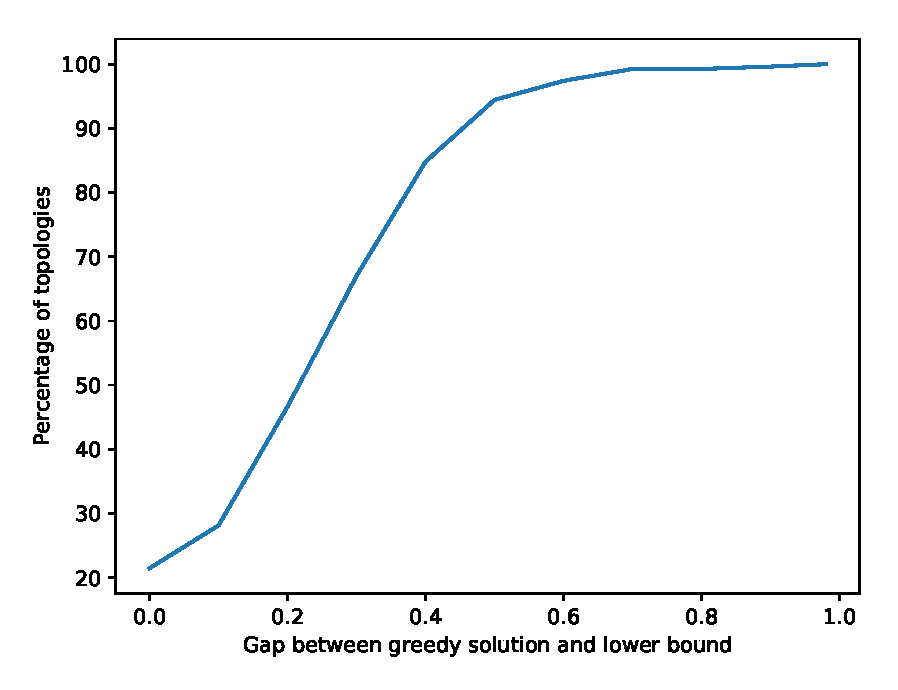
\includegraphics[width=.9\columnwidth]{./Network-lib/data/plot/minCycleCover_gapcdf.eps}
\end{center}
\caption{CDF of the gap between the greedy solution and the LP lower bound.}
\label{fig:cc_gap_cdf}
\end{figure}

The most important aspect is that by combining the minimum segment cost sr-cycle covers
with the column generation and the greedy algorithm we are able to greatly reduce the number of sr-cycles
in the minimum segment cost cover. Therefore, our solution is able to find sr-cycle covers that 
not only use the minimum amount of segments required for \emph{any} sr-cycle cover but also
are quite close to the minimum theoretical number of sr-cycles.
